\section{Implementation and results}

    \paragraph
    In this section, the techniques introduced in 
    Section~\ref{sec:param_estimation}, 
    \ref{sec:dmdc}, 
    and \ref{sec:havok} 
    will be applied to simulation data.
    Firstly, the influence of the design parameters on the algorithm performance will be discussed.
    These parameters include hyperparameters, the length of training data and the algorithm sample time.
    The effect of conditions that are not determined by algorithm design will also be explored, 
    like measurement noise, and the physical properties of the payload.
    Finally, the white-box and black-box techniques will be tested on a dynamic payload 
    which does not satisfy the assumptions of a simple pendulum.

    \subsection{Methodology} \label{sec:sys_id_methodology}

        \paragraph
        A \gls{SITL} implementation of the PX4 Autopilot \cite{Meier2015} using the Gazebo simulator \cite{Koenig2004} is used to generate data
        for system identification.
        Testing these techniques with simulation data allows us to investigate a much larger range of system configurations 
        than possible with practical flights.
        The simulation model used in Gazebo was verified in Chapter~\ref{chap:modelling}.
        Using PX4 in \gls{SITL} also ensures that the controller dynamics in simulation 
        is as close as possible to practical flights since the same flight stack is used in both cases.
        Gazebo applies realistic measurement noise to the signals received by PX4 
        and the PX4 flight stack applies an \gls{EKF} for state estimation.
        Therefore the the data seen by the system identification techniques 
        include the same \gls{EKF} filtering as practical flight data.

        \paragraph
        The procedure used to evaluate the black-box techniques is as follows:
        \begin{enumerate}
            \item Takeoff and hover with the multirotor
            \item Start logging input and output data
            \item Command a series of velocity step setpoints with random step sizes and time intervals
            \item Stop logging data
            \item Split data into separate training and testing periods
            \item Build a model from the training data
            \item Calculate an error metric for the model from the testing data
        \end{enumerate}

        \paragraph
        The default \gls{PID} velocity controller from PX4 is used during these simulation.
        The implemented controller gains are documented in Appendix~\ref{appen:pid_gains}.
        A \gls{ROS} node is used to read and log the payload angle measurement from Gazebo 
        and a different \gls{ROS} node is used to send velocity setpoints to PX4 
        with the MAVLink protocol through the popular \gls{ROS} package, 'mavros'.
        
        \paragraph
        A algorithm schedules the series of velocity step commands 
        by assigning random step values and time-intervals within a specified range.
        These values are selected from a uniform distribution 
        within the ranges specified in Table~\ref{tbl:input_ranges}
        The maximum velocity step is determined in simulation by iteratively increasing the maximum velocity step 
        to a safe value where the multirotor remains in stable flight
        and the payload angles do not swing out of control.
        The time interval range is set iteratively to ensure 
        that the generated data includes both transient and steady-state dynamics.
 
        \begin{table}[!h]
            \renewcommand{\arraystretch}{1.1}
            \centering
            \caption{Input data ranges.}
            \begin{tabularx}{0.65\linewidth}{@{}lCCr@{}}
                \toprule
                         & Velocity step [\SI{}{\metre/\second}]  & Step time interval [\SI{}{\second}]\\
                \midrule
                Minimum  & 0                                    & 10\\
                Maximum  & 3                                    & 25\\
                \bottomrule
            \end{tabularx}
            \label{tbl:input_ranges}
        \end{table}
        
        \begin{figure}[!htb]
    \centering
    \begin{tikzpicture}
        \begin{axis}[            
            xlabel = Time,
            ylabel = North velocity,
            x unit = \si{\second},
            y unit = \si{\radian},
            xmin = 0,   xmax = 200,
            ymin = -2.5,  ymax = 2.5,
            grid = major,
            legend cell align = left,
            legend pos = north east,
            grid style = dashed,
            legend style = {font = \scriptsize},
            label style = {font = \scriptsize},
            tick label style = {font = \scriptsize},
            width = 0.95\columnwidth,
            height = 0.5\columnwidth,
            % initialize Dark2
            cycle list/Dark2,
            % combine it with 'mark list*':
            cycle multiindex* list = {
                Dark2\nextlist
            }
        ]
        
        \addplot+[mark = none, style = solid, ultra thick] 
        table[x = time, y = vel_sp, col sep = comma] 
        {system_id/csv/training_data_SITL_x_vel_noise_l1_m0-2.csv.csv};
        \addlegendentry{$V_{N,sp}$}
        
        \addplot+[mark = none, style = solid, ultra thick] 
        table[x = time, y = vel, col sep = comma] 
        {system_id/csv/training_data_SITL_x_vel_noise_l1_m0-2.csv.csv};
        \addlegendentry{$V_N$}

        \end{axis}
    \end{tikzpicture} 
    
    \caption{Example of training data with random velocity step inputs
        ($m_p =$~\SI{0.2}{\kilo\gram}, $l =$~\SI{1}{\meter})}
    \label{fig:training_data}
\end{figure}


        \paragraph
        Figure~\ref{fig:training_data} 
        shows an example of random velocity steps and the resulting velocity response used as training data.
        Using random velocity steps and time intervals prevents the system identification methods 
        from overfitting to a specific set of control conditions.
        The method should rather determine a generalised model 
        that works over a range of possible control conditions.
        The data logged for the duration of the training data shows minimal altitude fluctuations.
        These fluctuations appear to be due to \gls{GPS} noise rather than the swinging payload, 
        since they do not show high freqeuncy osccilations as seen in the North velocity.
        This supports the assertion in \ref{sec:plant_considered} 
        that the considered plant approximates a pendulum-on-a-cart model during longitudinal control.

        % ?? Add plot and paragraph if there is time
        % \begin{figure}[!htb]
    \centering
    \begin{tikzpicture}
        \begin{axis}[            
            xlabel = Time,
            ylabel = North velocity,
            x unit = \si{\second},
            y unit = \si{\metre/\second},
            xmin = 0,   xmax = 200,
            ymin = -2.5,  ymax = 2.5,
            grid = major,
            legend cell align = left,
            legend pos = north east,
            grid style = dashed,
            legend style = {font = \scriptsize},
            label style = {font = \scriptsize},
            tick label style = {font = \scriptsize},
            width = 0.95\columnwidth,
            height = 0.5\columnwidth,
            % initialize Dark2
            cycle list/Dark2,
            % combine it with 'mark list*':
            cycle multiindex* list = {
                Dark2\nextlist
            }
        ]
        
        \addplot+[mark = none, style = solid, ultra thick] 
        table[x = time, y = vel_sp, col sep = comma] 
        {system_id/csv/training_data_SITL_x_vel_noise_l1_m0-2.csv.csv};
        \addlegendentry{$V_{N,sp}$}
        
        \addplot+[mark = none, style = solid, ultra thick] 
        table[x = time, y = vel, col sep = comma] 
        {system_id/csv/training_data_SITL_x_vel_noise_l1_m0-2.csv.csv};
        \addlegendentry{$V_N$}

        \end{axis}
    \end{tikzpicture} 
    
    \caption{Example of training data with random velocity step inputs
        ($m_p =$~\SI{0.2}{\kilo\gram}, $l =$~\SI{1}{\meter})}
    \label{fig:training_data_altitude}
\end{figure}


        % \paragraph
        % Figure~\ref{fig:training_data_altitude} shows the altitude of the multirotor during the training data period.
        % The multirotor does experience
        % This is due to speed of the altitude controllers

        \paragraph
        The data logged from simulation is then divided into testing and training data.
        The training data is used by the system identification algorithms to generate a regression model
        and the model is then used to determine a prediction error metric over the unseen testing data.
        It is common practice in model evaluations
        to use separate sets of data for training and testing.
        This ensures that good prediction scores do not result from models that overfit the training data. 
        
        \paragraph
        The testing data spans a fixed length of time and is taken from the start of the simulation period.
        The training data is then extracted from the remainder of the data.
        The same setpoint schedules are used to generate this data for different simulations
        to ensure that the metrics determined from different simulations are comparable. 
        The error metric calculated from the testing data is used to evaluate and rank the performances of each model.       
        % It is important to note that the testing data contains steps sizes and intervals not captured in the training data.
        % Write about generalisable models and that different steps sizes??
        % Edit this part ??

        % \paragraph
        % As discussed before, the purpose of identifying a data-driven model of the plant dynamics 
        % is to use it in a \gls{MPC} controller in the velocity loop, 
        % therefore velocity inputs are used in the system identification process.
        % It is a common technique to use a step response for system identification \cite{Chen2011} because it exposes a 
        % large range of frequency data in the system dynamics.
        % In other data-driven techniques like Neural-Nets, it may be helpful to use a larger variety of input types.
        % The input schedule may be generated by randomly switching between step, ramp and exponetional inputs 
        % to further gaurd againts overfitting \cite{Kotze2021}.
        % However, for the 
        % In practice it is more common to command position step setpoints since a multirotor delivers

    \subsection{Error metric}

        \paragraph        
        It is common practice is to select a model for a \gls{MPC} based on k-step-ahead prediction errors \cite{Zhao2014}.
        This is because the model is used to make k-step-ahead predictions during control optimisation.
        When model error is dominated by variance error (caused by disturbances), 
        it may be better to use one-step-prediction error \cite{Zhao2014}.
        However for the multirotor and payload case it is assumed that variance error 
        (caused by under modelling) dominates the model error.

        \paragraph
        Different metrics are used in literature to quantify prediction accuracy for different applications.
        Very common, scale-dependant error metrics are \gls{MSE} and MAE.
        These metrics are dependant on the unit and scale of a variable, 
        hence they cannot be used to compare predictions of different variables.
        \gls{MSE} ($l_2$~norm of error values) penalises larger errors more than smaller errors, 
        whereas MAE ($l_1$~norm) penalises errors equally.
        For our use case the $l_1$~norm provides a more intuitive metric than the $l_2$~norm
        because it has the same unit as the prediction variable
        and there is no motivation to penalise larger errors more than smaller errors for our use case.

        \paragraph
        MAE is calculated as:
        % \begin{equation}
        %     \bm{MAE} = \frac{1}{N_{run}} \cdot \sum_{k = 1}^{N_{run}} \left\lvert \bm{\hat{x_k}} - \bm{x_k} \right\rvert ,
        % \end{equation}
        \begin{equation}
            \bm{MAE} = mean \left( \phantom{.} \left\lvert \bm{\hat{x_k}} - \bm{x_k} \right\rvert \phantom{.} \right),
        \end{equation}
        where 
        % $N_{run}$ is the number of samples used in the prediction run,
        $\bm{MAE}$ is a vector with the MAE of each state,
        $\bm{x_k}$ is the actual state vector at time-step $k$, 
        $\bm{\hat{x_k}}$ is the state prediction, 
        and 
        $\bm{\hat{x_k}}$ is the state prediction.
        
        \paragraph
        Popular, scale-free error metrics, like \gls{MAPE}, \gls{MRAE} and \gls{MASE}, are also based on the $l_1$~norm,
        but are independent of the scale and units of a variable \cite{Hyndman2006}.
        These metrics could therefore be used to compare predictions of different variables.
        However, these metrics provide misleading comparisons for our use case.
        \gls{MAPE} expresses accuracy as the absolute ratio between the error and actual value at each time-step.
        This results in undefined or extremely large values for the payload angle predictions becasue the state has a zero mean.
        The velocity state variable has a non-zero mean, 
        therefore the scale of the \gls{MAPE} of velocity will significantly different from the \gls{MAPE} of the payload angle.
        
        \paragraph
        \gls{MRAE} is also popular metric for comparing predictions models used with a \gls{MPC} \cite{Kaiser2018b},
        however, similarly to \gls{MAPE}, it also results in undefined values for the payload swing angle.
        \gls{MASE} does not have this problem and can compare predictions of different variables well, 
        because it expresses accuracy as the ratio between the MAE of the model prediction and the MAE of an in-sample
        naive forecast \cite{Hyndman2006}.
        However, an in-sample forecast is a naive prediction for a one-step-ahead prediction, 
        but not for a k-step-ahead prediction.
        Therefore \gls{MASE} is not a helpful ratio for our use case.

        \paragraph
        \gls{NMAE} (Normalised Mean Absolute Error) is a scale-free error metric which provides a fair comparison of different variables in our use case.
        In this work \gls{NMAE} normalises the MAE of a variable by the range of that variable, 
        thereby variables with different ranges or different means can be compared.
        This value is calculated as:
        % \begin{equation}
        %     metric = \frac{1}{n_x} \cdot \sum_{i = 1}^{n_x} \left( \frac{ \bm{MAE_i} }{ x_{i, max} } \right) 
        % \end{equation}
        \begin{equation}
            NMAE = \frac{ MAE }{ x_{max} - x_{min} }
        \end{equation}
        where         
        $x_{i, max}$ and $x_{i, min}$ are the maximum and minimum values 
        of the considered variable in the testing data.
        % ?? Write about what this error means
        % ?? write that it is understood as percentage

        \paragraph
        This results in an error metric for each predicted variable, 
        but a single value is required per model 
        to rank the overall accuracy of different models.
        Therefore the average of the NMAE of all state variables
        is used as the single value representing the overall accuracy of a model
        and is denoted as $\overline{NMAE}$.
        This is the final error metric used to evaluate the model predictions 
        in the sections to follow.

        % \paragraph
        % Other considered error metrics are IAE and ITAE which adds up error over the prediction period.
        % IAE integrates the absolute error over time and weights all error equally.
        % ITAE integrates the absolute error multiplied by time over time 
        % hence errors that occur later in the prediction are weighted more than those that that occur earlier.
        % MAE was chosen over these metrics 
        % since it is closer to the loss function of the \gls{MPC} than IAE or ITAE.
        % Especially, ITAE achieves the opposite of what is desired because it penalises earlier errors less.
        % For the \gls{MPC} it is more important that early prediction errors are small since it will reoptimise later  

        \paragraph
        Other criteria which are more statistically rigorous in model selection 
        than error metrics are \gls{AIC} and \gls{BIC} scores.
        % These are information criteria scores which compute the maximum log likelihood of the model 
        % and add a penalty based on the number of terms in the model.
        Thereby they provide a quantitative way of performing a Pareto analysis, 
        which balances model complexity with model accuracy \cite{Mangan2017}.
        It is generally advantageous to use a parsimonious model, 
        which has a low prediction error but is not overly complex, 
        than a complex model with a slightly lower prediction error.
        This not only helps to avoid overfitting, but also ensures that the \gls{MPC} optimisation problem 
        is not too computational expensive for the available hardware.
        However, these scores require the computation of the maximum log likelihood of each model 
        over numerous simulations.
        This is computationally intractable and unpractical for our use case 
        because of the large number of hyperparameter combinations to compare, 
        as explained in Section~\ref{sec:hyperparameters}.
        Therefore an error metric will rather be used to evaluate model accuracy.
        
        % because it provides a good measure of a model prediction 
        % and it is computationally fast enough to perform a wide hyperparameter search.
        % \gls{AIC} or \gls{BIC} may be able to identify a slightly better model, 
        % but when used with the \gls{MPC} this slight improvement in prediction accuracy 
        % will result in a negligible improvement in control performance

        \paragraph
        The error metric of one model may change significantly
        different starting conditions or prediction horizons.
        The prediction horizon used for model analysis is selected as \SI{20}{\second}
        which is at least twice as long as the desired \gls{MPC} prediction horizon.
        Some models have very accurate transient predictions, but prove to be unstable over a longer time horizon.
        If the prediction horizon is too short, these models may score unreasonably low error metrics.
        Selecting these such a model could result in unstable control at certain control conditions.
        Therefore a long prediction horizon is used for testing so that marginally unstable models 
        are penalised heavily in model selection. 

        % \murray{Maybe insert example of good initial prediction but bad long term ??}

        \paragraph
        Different starting conditions also have a large influence on the prediction score of a model.
        Some models may accurately predict transient behaviour, 
        while being extremely bad at steady-state predictions.
        This would result in an \gls{MPC} controlling the plant well during the initial step response,
        but becoming unstable during steady-state control.
        In order to have a \gls{MPC} that can control the plant during the different stages of a flight, 
        a model needs to be selected with accurate predictions over a range of different control conditions.
        
        \paragraph
        Therefore the error metric needs to include predictions from multiple starting conditions in the testing data.
        The resulting testing procedure is to first specify a number of equispaced starting conditions within the testing data.
        The model is then run multiple times for the length of the prediction horizon, 
        stating with different initial conditions each time.
        The \gls{NMAE} is determined for each run, 
        whereafter the average of these scores gives the final \gls{NMAE} score of the model.
        In order to balance the variety of testing conditions with the computational time per error metric calculation, 
        10 prediction runs with different initial conditions used in the final \gls{NMAE} score. 
        
        % \paragraph
        % Each state error signal is scaled by the reciprocal of the maximum value of that state variable in the training data.
        % % This is to provide a better representative error when taking the mean of state variable errors.
        % This is to ensure that a scale difference in the variable types create a bias in the error metric.
        % For example, the multirotor velocity reaches values of \SI{3}{\metre/\second} but the payload swing angle has a maximum of only \SI[]{0.526}{\radian}.
        % The velocity prediction error is therefore inherently larger than the payload angle prediction error
        % and will bias the error metric towards favouring models with good velocity predictions.
        % The proposed scaled error metric ensures that the MAE of each state variable can be compared to each other.
        % It also provides an error metric that is better and unbiased representative of the model prediction performance across all state variables. 

    \subsection{Hyperparameters} \label{sec:hyperparameters}
        
        \paragraph
        As discussed in Section~\ref{sec:dmdc} and \ref{sec:havok} 
        \gls{DMDc} and \gls{HAVOKc} models are dependent on two hyperparameters: 
        the number of delay-coordinates, $q$, 
        and the \gls{SVD} truncation rank, $p$.
        For each system identification run with different system parameters or a different length of training data,
        a hyperparameter search is performed to find the combination of hyperparameters 
        that results the lowest prediction error.
        Firstly, a coarsely spaced grid search is performed with large intervals between tested hyperparameter values.
        The range of tested hyperparameters is then reduced and a finer hyperparameter search is performed.
        From numerous simulation iterations, the range of significant hyperparameter values is conservatively determined to be,
        \begin{equation}
            5 < q < 30, \phantom{--} 5 < p < 50
        \end{equation}.

        \begin{figure}[htb]
    \centering
    \begin{tikzpicture}
        \begin{axis}[            
            xlabel = {Number of delay-coordinates, $q$},
            ylabel = $\overline{NMAE}$ \phantom{~},
            % x unit = \si{\second},
            y unit = \%,
            xmin = 2,     xmax = 40,
            ymin = 3.2,  ymax = 6.5,
            grid = major,
            legend cell align = left,
            legend pos = north east,
            grid style = dashed,
            legend style = {font = \scriptsize},
            label style = {font = \scriptsize},
            tick label style = {font = \scriptsize},
            width = 0.95\columnwidth,
            height = 0.5\columnwidth,
            % initialize Dark2
            cycle list/Dark2,
            % combine it with 'mark list*':
            cycle multiindex* list = {
                Dark2\nextlist
            }
        ]

        \addplot+[mark = none, style = solid, ultra thick] 
        table[x = q, y expr = {\thisrow{NMAE_mean}*100}, col sep = comma] 
        {system_id/csv/NMAE_vs_q_SITL_x_vel_noise_longer_times_q.csv_dmd_angle_Ttrain_60.csv};
        \addlegendentry{DMD}
        
        \addplot+[mark = none, style = solid, ultra thick] 
        table[x = q, y expr = {\thisrow{NMAE_mean}*100}, col sep = comma] 
        {system_id/csv/NMAE_vs_q_SITL_x_vel_noise_longer_times_q.csv_havok_angle_Ttrain_60.csv};
        \addlegendentry{HAVOK}

        \end{axis}
    \end{tikzpicture} 
    
    \caption{\gls{DMD} and \gls{HAVOK} predictions error for different lengths of noisy training data
    ($m_p =$~\SI{0.2}{\kilo\gram}, $l =$~\SI{0.5}{\meter}, $T_s =$~\SI{0.03}{\second}, $T_{train} =$~\SI{60}{\second}.)}
    \label{fig:NMAE_vs_q}
\end{figure}
 

        \paragraph
        Figure~\ref{fig:NMAE_vs_q} shows the prediction error of \gls{DMDc} and \gls{HAVOKc} models for different values of $q$.
        For each value of a $q$, a new model is generated with every $p$ in the considered range 
        and the lowest prediction error is plotted.
        There is only a slight difference between the results of \gls{DMDc} and \gls{HAVOKc}.
        As expected, the models with the least number of terms have the highest prediction errors.
        As the number of terms available to the model increases, the error decreases.
        It is clear that there is a sharp decrease in prediction error for $2 < q < 6$, 
        however there is no longer a significant decrease in error
        as model complexity increases past $q > 12$.        

        \paragraph
        This `elbow' in the plot can be considered as the Pareto front, 
        where there is a balance between model complexity and accuracy \cite{Mangan2017}.
        It is desirable to select a parsimonious model on this front that has just enough free parameters 
        to capture the plant dynamics and have good accuracy, 
        without being overly complex \cite{Brunton2019b}.
        These models are less prone to overfitting 
        and also lead to lower computational complexity in the \gls{MPC} optimisation problem.        

        \begin{figure}[htb]
    \centering
    \begin{tikzpicture}
        \begin{semilogyaxis}[            
            xlabel = Index of mode,
            ylabel = Singular value,
            % x unit = \si{\second},
            % y unit = \si{\second},
            xmin = 0,     xmax = 60,
            ymin = 1e-2,  ymax = 1e3,
            grid = major,
            legend cell align = left,
            legend pos = north east,
            grid style = dashed,
            legend style = {font = \scriptsize},
            label style = {font = \scriptsize},
            tick label style = {font = \scriptsize},
            width = 0.95\columnwidth,
            height = 0.5\columnwidth,
            % initialize Dark2
            cycle list/Dark2,
            % combine it with 'mark list*':
            cycle multiindex* list = {
                Dark2\nextlist
            }
        ]

        \addplot+[only marks, mark = square, ultra thick] 
        table[x = index, y = S, col sep = comma] 
        {system_id/csv/Singular_values_SITL_x_vel_noise_longer_times_q.csv_havok_angle_Ttrain_60_q29_p13.csv};
        \addlegendentry{Significant modes}

        \addplot+[only marks, mark = square, ultra thick] 
        table[x = index, y = S, col sep = comma] 
        {system_id/csv/Singular_values_SITL_x_vel_noise_longer_times_q.csv_havok_angle_Ttrain_60_q29_p13_trunc.csv};
        \addlegendentry{Truncated modes}

        \end{semilogyaxis}
    \end{tikzpicture} 
    
    \caption{Significant and truncated singular values of a \gls{HAVOKc} model produced from noisy data
    ($m_p =$~\SI{0.2}{\kilo\gram}, $l =$~\SI{0.5}{\meter}, $T_s =$~\SI{0.03}{\second}, $T_{train} =$~\SI{60}{\second}.).}
    \label{fig:singular_values}
\end{figure}


        \paragraph
        Figure~\ref{fig:singular_values} plots the singular values of the \gls{SVD} from a \gls{HAVOKc} model in a log scale.
        The singular values of the \gls{SVD} can be loosely interpreted as 
        a measure of significance of the corresponding \gls{POD} mode to the plant dynamics \cite{Brunton2019d}. 
        That is, modes with higher singular values contain more relevant information about the plant dynamics 
        than modes with lower singular values.
        The $p$ number of significant singular values, 
        which correspond to the \gls{POD} modes used to reconstruct the observed dynamics,
        are specifically shown in the plot.
        The truncated singular values are also shown, which correspond to the discarded modes.
        
        \paragraph
        The Pareto `elbow' is also visible in this plot where there is noticeable change in gradient
        roughly at the split between significant and truncated values.
        This change in gradient shows that after $p$ modes, 
        there is a significant drop in information contributed per remaining mode.
        Note that the number $p$ was selected from a hyperparameter search using an error metric
        which did not consider the singular values.
        This seems to confirm the notion that the Pareto optimal solution 
        is often the most accurate representation of the actual dynamics \cite{Brunton2019d}.

    \subsection{Sample time} \label{sec:sample_time}

        \paragraph
        The sample time, $T_s$, used for system identification is the sample time of the discrete model, 
        which determines the sample time of the \gls{MPC}.
        Resampling strategies can enable the \gls{MPC} to run at a different frequency to the discrete model 
        but this adds unnecessary complexity to the control architecture.
        
        \paragraph
        The \gls{MPC} acts in the velocity loop and commands an acceleration setpoint.
        The default \gls{PID} velocity controller runs at \SI{50}{\hertz} which corresponds to $T_s =~$\SI{0.02}{\second}.
        Due to the computational complexity of an \gls{MPC}, the optimiser will struggle to run at \SI{50}{\hertz} on a companion computer on a multirotor.
        However, the controller needs to run as fast as possible 
        to have significant time-scale separation from the multirotor dynamics.
        If the controller runs too slowly, it may result in poor flight performance or unstable control.
        The highest natural frequency of the payload based on the range of physical parameters considered 
        is~\SI{8.39}{\hertz} corresponding to a period of \SI{0.119}{\second}.

        \begin{figure}[htb]
    \centering
    \begin{tikzpicture}
        \begin{axis}[            
            xlabel = Ts,
            ylabel = NMAE\textsubscript{mm},
            % x unit = \si{\second},
            % y unit = \si{\second},
            xmin = 0.02,  xmax = 0.05,
            ymin = 0.03,  ymax = 0.055,
            grid = major,
            legend cell align = left,
            legend pos = north east,
            grid style = dashed,
            legend style = {font = \scriptsize},
            label style = {font = \scriptsize},
            tick label style = {font = \scriptsize},
            width = 0.45\columnwidth,
            height = 0.5\columnwidth,
            % initialize Dark2
            cycle list/Dark2,
            % combine it with 'mark list*':
            cycle multiindex* list = {
                Dark2\nextlist
            }
        ]

        % \addplot+[mark = none, style = solid, ultra thick] 
        % table[x = Ts, y = NMAE_mean, col sep = comma] 
        % {system_id/csv/NMAE_vs_Ts_SITL_x_vel_noise_l0-25_m0-2.csv_dmd_angle.csv};
        % \addlegendentry{$l =$~\SI{0.25}{\metre}}
        
        \addplot+[mark = none, style = solid, ultra thick] 
        table[x = Ts, y = NMAE_mean, col sep = comma] 
        {system_id/csv/NMAE_vs_Ts_SITL_x_vel_noise_l0-5_m0-2.csv_dmd_angle.csv};
        \addlegendentry{$l =$~\SI{0.5}{\metre}}
        
        \addplot+[mark = none, style = solid, ultra thick] 
        table[x = Ts, y = NMAE_mean, col sep = comma] 
        {system_id/csv/NMAE_vs_Ts_SITL_x_vel_noise_l1_m0-2.csv_dmd_angle.csv};
        \addlegendentry{$l =$~\SI{1}{\metre}}
        
        \addplot+[mark = none, style = solid, ultra thick] 
        table[x = Ts, y = NMAE_mean, col sep = comma] 
        {system_id/csv/NMAE_vs_Ts_SITL_x_vel_noise_l2_m0-2.csv_dmd_angle.csv};
        \addlegendentry{$l =$~\SI{2}{\metre}}
        
        \end{axis}
    \end{tikzpicture} 
    
    \caption{DMD prediction error using different cable lengths with a range of different sample times of noisy training data
    ($m =$~\SI{0.2}{\kilo\gram})}
    \label{fig:MAE_vs_Ts_vs_L}
\end{figure}


        \paragraph
        Figure~\ref{fig:MAE_vs_Ts_vs_L} shows the prediction error of different \gls{DMDc} models 
        generated with a range of different sample times.
        The natural frequency of the payload pendulum is dependant on the cable length 
        and influences the frequency response of the plant.
        Therefore Figure~\ref{fig:MAE_vs_Ts_vs_L} plots the experiment result 
        for different cable lengths to see if it has an effect on the prediction error of the models.

        \paragraph
        % It appears that for $l =$~\SI{0.25}{\metre}, the prediction error increases for larger sample times.
        % This is because the shorter cable length results in a higher natural frequency of the payload,
        % hence a faster sample time is required for accurate system identification.
        Note that for all considered cable lengths, the prediction error has a sharp decrease for 
        $T_s >$~\SI{0.045}{\second}.
        This may be because the model does not try to capture the small, high-frequency oscillations in the dynamics
        at such slow sample times.
        Hence the long term prediction of the models fits the general shape of the dynamics well and results in low errors.
        However, this sample time is too slow for controlling the practical multirotor.
        $T_s =$~\SI{0.03}{\second} is selected as the sample time for system identification 
        because it provides a good balance between being fast enough for the multirotor dynamics and slow enough for a practical \gls{MPC} implementation.

    \subsection{Choice of payload variable in the state vector} \label{sec:payload_state_variable}

        \paragraph
        As discussed in Section~\ref{sec:plant_considered}, 
        the equations of motion in continuous-time of a floating pendulum are dependent on $\dot{\theta}$ and $V_N$, 
        but are not dependent on $\theta$.
        Therefore it is expected that 
        $
        \bm{x} = \begin{bmatrix}
            V_N & \dot{\theta}
        \end{bmatrix}^T
        $
        will be used as the state vector for system identification.
        However, if $\dot{\theta}$ is not included in the state vector of a discrete model, 
        it can still be represented with numerical differentiation of $\theta$.
        An example of this is the backward Euler form,
        \begin{equation}
            \dot{\theta}_k = (\frac{1}{T_s}) \cdot \theta_k - (\frac{1}{T_s}) \cdot \theta_{k-1} .
        \end{equation}
        Therefore the original state vector can also be replaced by,
        $
            \bm{x} = \begin{bmatrix}
                V_N & \theta
            \end{bmatrix}^T
        $
        for system identification.

        \paragraph
        Based on the floating pendulum equations, it is expected that a model derived from $\dot{\theta}$ data 
        will better approximate the actual dynamics than one using $\theta$.
        This is because $\dot{\theta}$ is directly related to the dynamics, 
        compared to $\theta$ which needs to be related to $\dot{\theta}$ to be relevant for the dynamics.
        However, an experiment to compare the performances of these models shows that this has a  negligible effect.

        \begin{figure}[h]
    \centering
    \begin{tikzpicture}
        \begin{axis}[            
            xlabel = Length of training data,
            ylabel = MAE of North velocity prediction,
            x unit = \si{\second},
            % y unit = \si{\second},
            xmin = 0,     xmax = 100,
            ymin = 0.14, ymax = 0.28,
            grid = major,
            legend cell align = left,
            legend pos = north east,
            grid style = dashed,
            legend style = {font = \scriptsize},
            label style = {font = \scriptsize},
            tick label style = {font = \scriptsize},
            width = 0.95\columnwidth,
            height = 0.5\columnwidth,
            % initialize Dark2
            cycle list/Dark2,
            % combine it with 'mark list*':
            cycle multiindex* list = {
                Dark2\nextlist
            }
        ]
         
        \addplot+[mark = none, style = solid, ultra thick] 
        table[x = T_train, y = MAE_1, col sep = comma] 
        {system_id/csv/MAE_vs_Ntrain_SITL_x_vel_noise_l1_m0-2_state_vector.csv_havok_angle.csv};
        \addlegendentry{Using $\bm{\theta}$}
        
        \addplot+[mark = none, style = dashed, ultra thick] 
        table[x = T_train, y = MAE_1, col sep = comma] 
        {system_id/csv/MAE_vs_Ntrain_SITL_x_vel_noise_l1_m0-2_state_vector.csv_havok_angular_rate.csv};
        \addlegendentry{Using $\bm{\dot{\theta}}$}

        % \addlegendentry{HAVOK with $\theta$ and $\dot{\theta}$}

        \end{axis}
    \end{tikzpicture} 
    
    \caption{Prediction MAE for HAVOK models using either angle or angular rate measurements 
    ($m =$~\SI{0.2}{\kilo\gram}, $l =$~\SI{1}{\meter}, $T_s =$~\SI{0.03}{\second}).}
    \label{fig:SITL_MAE_vs_train_angular_rate}
\end{figure}


        \paragraph
        Figure~\ref{fig:different_state_vectors} shows the prediction error of \gls{HAVOKc} models using $\dot{\theta}$ or $\theta$ 
        for a range training data lengths.
        Only for very short lengths of training data, do models using $\dot{\theta}$ outperform those using $\theta$.
        For longer lengths of training data there is a negligible difference in prediction error between the methods.
        Therefore $\theta$ will be used for system identification to avoid unnecessary complexity, 
        since there is no direct measurement of $\dot{\theta}$ on the practical multirotor.

    \subsection{Noise} \label{sec:noise}

        \paragraph
        Measurement noise is bad for system identification because it adds high-frequency information to the output signals
        which are not part of the actual dynamics.
        On the practical multirotor the \gls{IMU}, barometer, magnetometer and \gls{GPS} sensors experience measurement noise.
        The \gls{EKF} performs sensor fusion and smooths out most of the measurement noise 
        to provide a state estimate that is less noisy than raw sensor values.
        Therefore the output from the \gls{EKF} is used for system identification.
        
        \paragraph
        The potentiometer and \gls{ADC} which measure the payload angle on the multirotor also has experience measurement noise.
        This signal is not smoothed by an onboard \gls{EKF}.
        In simulation noise is applied to the payload angle as band-limited white-noise.
        The applied noise power was iteratively adjusted to match that of the practical payload measurements.
        The noisy signals from both the multirotor \gls{EKF} and payload swing angle are smoothed 
        with a quadratic regression smoother from MATLAB\textsuperscript{\textregistered} before applying system identification.
        The smoother uses a fixed window length of 20 samples which was selected iteratively 
        to remove high-frequency variation without loosing the general shape of the data.

        \begin{figure}[!htb]
    \centering
    \begin{tikzpicture}
        \begin{axis}[            
            xlabel = Time,
            ylabel = North acceleration setpoint,
            x unit = \si{\second},
            y unit = \si{\metre/\second^2},
            xmin = 100,   xmax = 200,
            ymin = -2,  ymax = 2,
            grid = major,
            legend cell align = left,
            legend pos = north east,
            grid style = dashed,
            legend style = {font = \scriptsize},
            label style = {font = \scriptsize},
            tick label style = {font = \scriptsize},
            width = 0.95\columnwidth,
            height = 0.3\columnwidth,
            % initialize Dark2
            cycle list/Dark2,
            % combine it with 'mark list*':
            cycle multiindex* list = {
                Dark2\nextlist
            }
        ]
        
        \addplot+[mark = none, style = solid, ultra thick] 
        table[x = time, y = acc_sp, col sep = comma] 
        {system_id/csv/acc_sp_offset_SITL_x_vel_noise_l1_m0-2.csv.csv};
        % \addlegendentry{$A_{N,sp}$}

        \end{axis}
    \end{tikzpicture} 
    
    \caption{Accelleration setpoint training data from random velocity step inputs
        ($m =$~\SI{0.2}{\kilo\gram}, $l =$~\SI{1}{\meter})}
    \label{fig:acc_sp}
\end{figure}

        
        \paragraph
        The input signal also needs to be smoothed to remove high-frequency noise from the logged signal.
        The quadratic regression smoother does not fit the shape of the input data well 
        because of the sharp, non-differentiable edges in the acceleration setpoint signal.
        Therefore a Gaussian-weighted moving average smoother 
        from MATLAB\textsuperscript{\textregistered} is used for the input signal.
        
        \paragraph
        Figure~\ref{fig:acc_sp} shows the North acceleration setpoint for a period of training data.
        Without noise the acceleration setpoint should have a zero mean, 
        however the signal mean shows a constant offset.
        % This offset may be due to the integrators in the controllers correcting for an \gls{CoM} imbalance to keep the vehicle steady.
        The is due to a measurement offset in the \gls{IMU} which causes a offset in the orientation vector 
        and therefore affects the control signals.
        The setpoint mean is calculated from the training data and subtracted from the signal to correct for the offset.
        This results in a input signal with a zero mean.
        The calculated mean is reapplied to the \gls{MPC} control signal during implementation
        to readjust for the required offset.

        % \paragraph
        % However, since there is no direct measurement of $\dot{\theta}$, 
        % numerical differentiation is performed on the noisy $\theta$ measurement to estimate $\dot{\theta}$. 
        % This amplifies the noise and results in inaccurate $\dot{\theta}$ signal.
        % Total variation differentiation is implemented to estimate $\dot{\theta}$ from the noisy measurements more accurately.
        % Figure~\ref{fig:payload_noise_diff} shows
        
        % \input{system_id/plots/payload_noise_diff.tex} // With TVDiff 
        
        \begin{figure}[htb]
    \centering
    \begin{tikzpicture}
        \begin{axis}[            
            xlabel = Length of training data,
            ylabel = $\overline{NMAE}$ \phantom{~},
            x unit = \si{\second},
            y unit = \%,
            xmin = 5,     xmax = 120,
            ymin = 3.2,  ymax = 5.7,
            grid = major,
            legend cell align = left,
            legend pos = north east,
            grid style = dashed,
            legend style = {font = \scriptsize},
            label style = {font = \scriptsize},
            tick label style = {font = \scriptsize},
            width = 0.95\columnwidth,
            height = 0.5\columnwidth,
            % initialize Dark2
            cycle list/Dark2,
            % combine it with 'mark list*':
            cycle multiindex* list = {
                Dark2\nextlist
            }
        ]

        \addplot+[mark = none, style = solid, ultra thick] 
        table[x = T_train, y expr = {\thisrow{NMAE_mean}*100}, col sep = comma] 
        {system_id/csv/NMAE_vs_Ntrain_SITL_x_vel_no_noise_longer_times.csv_havok_angle.csv};
        \addlegendentry{Without noise}

        \addplot+[mark = none, style = solid, ultra thick] 
        table[x = T_train, y expr = {\thisrow{NMAE_mean}*100}, col sep = comma] 
        {system_id/csv/NMAE_vs_Ntrain_SITL_x_vel_noise_longer_times.csv_havok_angle.csv};
        \addlegendentry{With noise}

        \end{axis}
    \end{tikzpicture} 
    
    \caption{\gls{HAVOK} prediction errors for different lengths of training data with and without noise 
    ($m_p =$~\SI{0.2}{\kilo\gram}, $l =$~\SI{0.5}{\meter}, $T_s =$~\SI{0.03}{\second}).}
    \label{fig:noise_vs_no_noise}
\end{figure}


        Figure~\ref{fig:noise_vs_no_noise} compares the prediction errors of \gls{HAVOKc} models generated from data with or without noise.
        The plot shows that when using short lengths of training data, 
        the prediction errors are smaller for model generated with noiseless signals.
        However, it appears that the prediction errors are almost equal with longer lengths of training data.
        This is because with a short length of data, the signal variation or energy contributed of the noise is a significant part of the data
        and has a strong influence on the model.
        However, with longer lengths of data, the variation caused by the actual plant dynamics 
        dominates the low energy contribution of the measurement noise. 
        Hence, the noise has a smaller influence on the model.        
        It also appears that at long training data lengths noise has a negligible effect on the prediction error of the resulting models.

        \begin{figure}[htb]
    \centering
    \begin{tikzpicture}
        \begin{axis}[            
            xlabel = Length of training data,
            ylabel = $\overline{NMAE}$ \phantom{~},
            x unit = \si{\second},
            y unit = \%,
            xmin = 5,     xmax = 120,
            ymin = 3.2,  ymax = 5.7,
            grid = major,
            legend cell align = left,
            legend pos = north east,
            grid style = dashed,
            legend style = {font = \scriptsize},
            label style = {font = \scriptsize},
            tick label style = {font = \scriptsize},
            width = 0.95\columnwidth,
            height = 0.5\columnwidth,
            % initialize Dark2
            cycle list/Dark2,
            % combine it with 'mark list*':
            cycle multiindex* list = {
                Dark2\nextlist
            }
        ]

        \addplot+[mark = none, style = solid, ultra thick] 
        table[x = T_train, y expr = {\thisrow{NMAE_mean}*100}, col sep = comma] 
        {system_id/csv/NMAE_vs_Ntrain_SITL_x_vel_noise_longer_times.csv_dmd_angle.csv};
        \addlegendentry{DMD}

        \addplot+[mark = none, style = solid, ultra thick] 
        table[x = T_train, y expr = {\thisrow{NMAE_mean}*100}, col sep = comma] 
        {system_id/csv/NMAE_vs_Ntrain_SITL_x_vel_noise_longer_times.csv_havok_angle.csv};
        \addlegendentry{HAVOK}

        \end{axis}
    \end{tikzpicture} 
    
    \caption{\gls{DMD} and \gls{HAVOK} prediction errors for different lengths of noisy training data
    ($m_p =$~\SI{0.2}{\kilo\gram}, $l =$~\SI{0.5}{\meter}, $T_s =$~\SI{0.03}{\second}).}
    \label{fig:havok_vs_dmd_noise}
\end{figure}


        Figure~\ref{fig:havok_vs_dmd_noise} compares the performance of \gls{HAVOKc} and \gls{DMDc} model when using noisy data.
        The prediction error curves of the two methods are very simlar, with \gls{HAVOKc} producing slightly lower prediction errors than \gls{DMDc}.
        However, this difference in error may be so small that it has a negligible effect on control.  

    \subsection{System parameters} \label{sec:system_params}
            
        \paragraph
        The suspended payload, as described in Section~\ref{sec:plant_considered},
        has two system parameters, $m_p$ and $l$.
        For the practical multirotor considered, the payload mass is limited to,
        $
            0.1 \leq m_p \leq \SI{0.3}{\kilo\gram} ,
        $
        and the cable length is limited to:
        $
            0.5 \leq l \leq \SI{2}{\metre} .
        $
        Figure~\ref{fig:system_param_subfigs} shows the prediction error of \gls{HAVOKc} models 
        build from simulations with various values of $m_p$ and $l$.
        The plots are not shown for \gls{DMDc} models because they are so similar to the \gls{HAVOKc} results.

        
\begin{figure}
    \captionsetup[subfigure]{justification=centering}
    \centering
    \begin{subfigure}{0.45\columnwidth}
    \centering
    \begin{tikzpicture}
        \begin{axis}[            
            xlabel = Length of training data,
            ylabel = $\overline{NMAE}$ \phantom{~},
            x unit = \si{\second},
            y unit = \%,
            xmin = 0,     xmax = 120,
            ymin = 3,  ymax = 5.5,
            grid = major,
            legend cell align = left,
            legend pos = north east,
            grid style = dashed,
            legend style = {font = \scriptsize},
            label style = {font = \scriptsize},
            tick label style = {font = \scriptsize},
            width = 0.9\columnwidth,
            height = 0.9\columnwidth,
            % initialize Dark2
            cycle list/Dark2,
            % combine it with 'mark list*':
            cycle multiindex* list = {
                Dark2\nextlist
            }
        ]
        
        \addplot+[mark = none, style = solid, ultra thick] 
        table[x = T_train, y expr = {\thisrow{NMAE_mean}*100}, col sep = comma] 
        {system_id/csv/NMAE_vs_Ntrain_SITL_x_vel_noise_l0-5_m0-2.csv_havok_angle.csv};
        \addlegendentry{$l =$~\SI{0.5}{\metre}}
        
        \addplot+[mark = none, style = solid, ultra thick] 
        table[x = T_train, y expr = {\thisrow{NMAE_mean}*100}, col sep = comma] 
        {system_id/csv/NMAE_vs_Ntrain_SITL_x_vel_noise_l1_m0-2.csv_havok_angle.csv};
        \addlegendentry{$l =$~\SI{1}{\metre}}
        
        \addplot+[mark = none, style = solid, ultra thick] 
        table[x = T_train, y expr = {\thisrow{NMAE_mean}*100}, col sep = comma] 
        {system_id/csv/NMAE_vs_Ntrain_SITL_x_vel_noise_l2_m0-2.csv_havok_angle.csv};
        \addlegendentry{$l =$~\SI{2}{\metre}}
        
        \end{axis}
    \end{tikzpicture} 
    
    \caption{$m_p = $~\SI{0.2}{\kilo\gram}, with varying $l$}
    \label{fig:different_lengths}
\end{subfigure}
 % subfigure
    \begin{subfigure}{0.45\columnwidth}
    \centering
    \begin{tikzpicture}
        \begin{axis}[            
            xlabel = Length of training data,
            ylabel = $\overline{NMAE}$ \phantom{~},
            x unit = \si{\second},
            y unit = \%,
            xmin = 0,     xmax = 120,
            ymin = 3,  ymax = 5.5,
            grid = major,
            legend cell align = left,
            legend pos = north east,
            grid style = dashed,
            legend style = {font = \scriptsize},
            label style = {font = \scriptsize},
            tick label style = {font = \scriptsize},
            width = 0.9\columnwidth,
            height = 0.9\columnwidth,
            % initialize Dark2
            cycle list/Dark2,
            % combine it with 'mark list*':
            cycle multiindex* list = {
                Dark2\nextlist
            }
        ]
         
        \addplot+[mark = none, style = solid, ultra thick] 
        table[x = T_train, y expr = {\thisrow{NMAE_mean}*100}, col sep = comma] 
        {system_id/csv/NMAE_vs_Ntrain_SITL_x_vel_noise_l1_m0-1.csv_havok_angle.csv};
        \addlegendentry{$m_p =$~\SI{0.1}{\kilo\gram}}
        
        \addplot+[mark = none, style = solid, ultra thick] 
        table[x = T_train, y expr = {\thisrow{NMAE_mean}*100}, col sep = comma] 
        {system_id/csv/NMAE_vs_Ntrain_SITL_x_vel_noise_l1_m0-2.csv_havok_angle.csv};
        \addlegendentry{$m_p =$~\SI{0.2}{\kilo\gram}}
        
        \addplot+[mark = none, style = solid, ultra thick] 
        table[x = T_train, y expr = {\thisrow{NMAE_mean}*100}, col sep = comma] 
        {system_id/csv/NMAE_vs_Ntrain_SITL_x_vel_noise_l1_m0-3.csv_havok_angle.csv};
        \addlegendentry{$m_p =$~\SI{0.3}{\kilo\gram}} 
        
        \end{axis}
    \end{tikzpicture} 

    \caption{$l = $~\SI{1}{\metre}, with varying $m_p$}
    \label{fig:different_masses}
\end{subfigure}
 % subfigure
    \caption{\gls{HAVOK} prediction errors for different system parameters}
    \label{fig:system_param_subfigs}  
\end{figure}

        From Figure~\ref{fig:different_lengths} it seems that there is not a great difference in prediction error 
        for different cable length setups.
        From Figure~\ref{fig:different_masses} it appears that $m_p$ has a greater effect on prediction error,
        since there is a bigger difference in prediction error between plots of different $m_p$ values.
        However, it is clear that the system identification method works for a range of different payload parameters.

        % When no external payload is attached, the connection device attached to the end of the cable is 
        % $m_p = \SI{0.01}{\kilo\gram}$.
        % % It becomes unsafe to Flying without a cable attached to the cable, or with a payload with a very small mass, 
        % % may become unsafe since the cable may not always  kept taut by the mass. 
        % On the other limit, $m_p = \SI{0.4}{\kilo\gram}$ is determined to be the maximum payload mass the multirotor can carry safely 
        % based on the maximum thrust of the motors.

        % A cable length shorter than \SI{0.5}{\metre} is quite impractical and may rather be attached as a rigid payload.
        % There are very few practical applications that may require a shorter cable length.
        % It is also unsafe to fly with a shorter cable length, 
        % since the payload may collide with the multirotor during an uncontrolled swing.
        % A longer cable guards against a payload and vehicle collision, 
        % because more energy needs to be transferred to the payload to reach the height of the vehicle. 
        % The maximum cable length is selected as $l=~\SI{2}{\metre}$ by intuition 
        % since a cable much longer than this may not be practically useful for a drone delivery flight with the considered multirotor.

    \subsection{Length of training data} \label{sec:sys_id_length_of_data}
    
        \paragraph
        From the plots discussed in previous sections, 
        it is obvious that the accuracy of a model is dependant 
        on the length of training data exposed to the system identification algorithm.
        The general relationship between length of training data and prediction error 
        is illustrated in Figure~\ref{fig:system_param_subfigs}.
        For very short lengths of training data the prediction error is large, 
        but as training length increases, the prediction error improves up to a point.
        After this point, the prediction error slowly worsens with increasing lengths of training data.
        
        \paragraph
        This trend may be counter-intuitive, because it is generally expected that more training data leads to better models.
        The logic follows that more training data leads to less overfitting 
        which leads to better test data predictions.
        However, a phenomenon named `double-descent' occurs when the dimension of a regression model, $D$ 
        is near the number of training samples, $N_{train}$ \cite{Nakkiran2019}.
        In this critical region at the transition between over-parameterized and under-parameterized models,
        the prediction error initially decreases, then increases to a peak whereafter it decreases again \cite{Nakkiran2019}. 
        
        \paragraph
        A rough calculation confirms that the critical region of `double-descent' is applicable to our use case.
        The highest $q$ in the considered range is 30, which corresponds to a model dimension of 
        \begin{equation}
            D = (q \cdot n_x)^2 + (q \cdot n_x)(n_u) = 3660 .
        \end{equation}
        The length of training data corresponding to $D = N_{train} \cdot n_x$ at the transition between over- and under-parameterization is therefore:
        \begin{equation}
            T_{train} = N_{train} \cdot T_s = \SI{54.9}{\second} .
        \end{equation}
        This value is indeed within the range of considered training data lengths,
        which explains why our training experiments experience this phenomenon.

        \paragraph
        It should be noted that the plot for $l =$~\SI{0.5}{\metre} in Figure~\ref{fig:different_lengths}
        does not follow the `double-descent' trend.
        This may be because the short cable length corresponds to large swing angles and a high natural frequency.
        The onboard \gls{PID} controllers do not damp these oscillations as quickly 
        as the smaller angle and lower frequency oscillations of longer cables.
        Hence there is not enough information exposed in the first few step responses of the training data and
        the algorithm needs more step responses to accurately capture the steady-state behaviour of the plant.

        \paragraph
        In a practical implementations, training data is costly and it is desirable to use less training data.
        Less training data means less flight time will be wasted on training a model before the multirotor can fly with a updated controller.
        Less training data also corresponds to lower memory usage on the multirotor hardware and lower time-complexity for the algorithm.
        Therefore it is not practical to increase the amount of training data to the under-parameterized region.
        Hence, the critical region of training data lengths will be used and
        the data length corresponding to the lowest prediction error will be selected per simulation.

    \subsection{Dynamic payload} \label{sec:dynamic_payload}
        
        \paragraph
        In Section~\ref{sec:param_estimation} it was shown that the white-box system identification method
        perform well for the suspended payload use case.
        It was also shown in \cite{Slabber2020} and \cite{Erasmus2020} that this method can be used 
        in conjunction with \gls{LQR} control to minimize swing angles of an unknown payload.
        However, many payloads do not satisfy the assumptions made in for the a priori model
        which is detrimental to performance of white-box method.
        For example, for an elongated payload attached to the cable the point-mass assumption does not hold.
        The \gls{CoM} of the payload is well below the attachment point of the cable, 
        which creates a double pendulum model that differs significantly from a simple pendulum.
        Such a payload is better represented in \gls{2D} by the double pendulum modelled in Figure~\ref{fig:double_pend}, 
        than the model defined in Figure~\ref{fig:floating_pend}.

        \begin{figure}[htb]
            \centering
            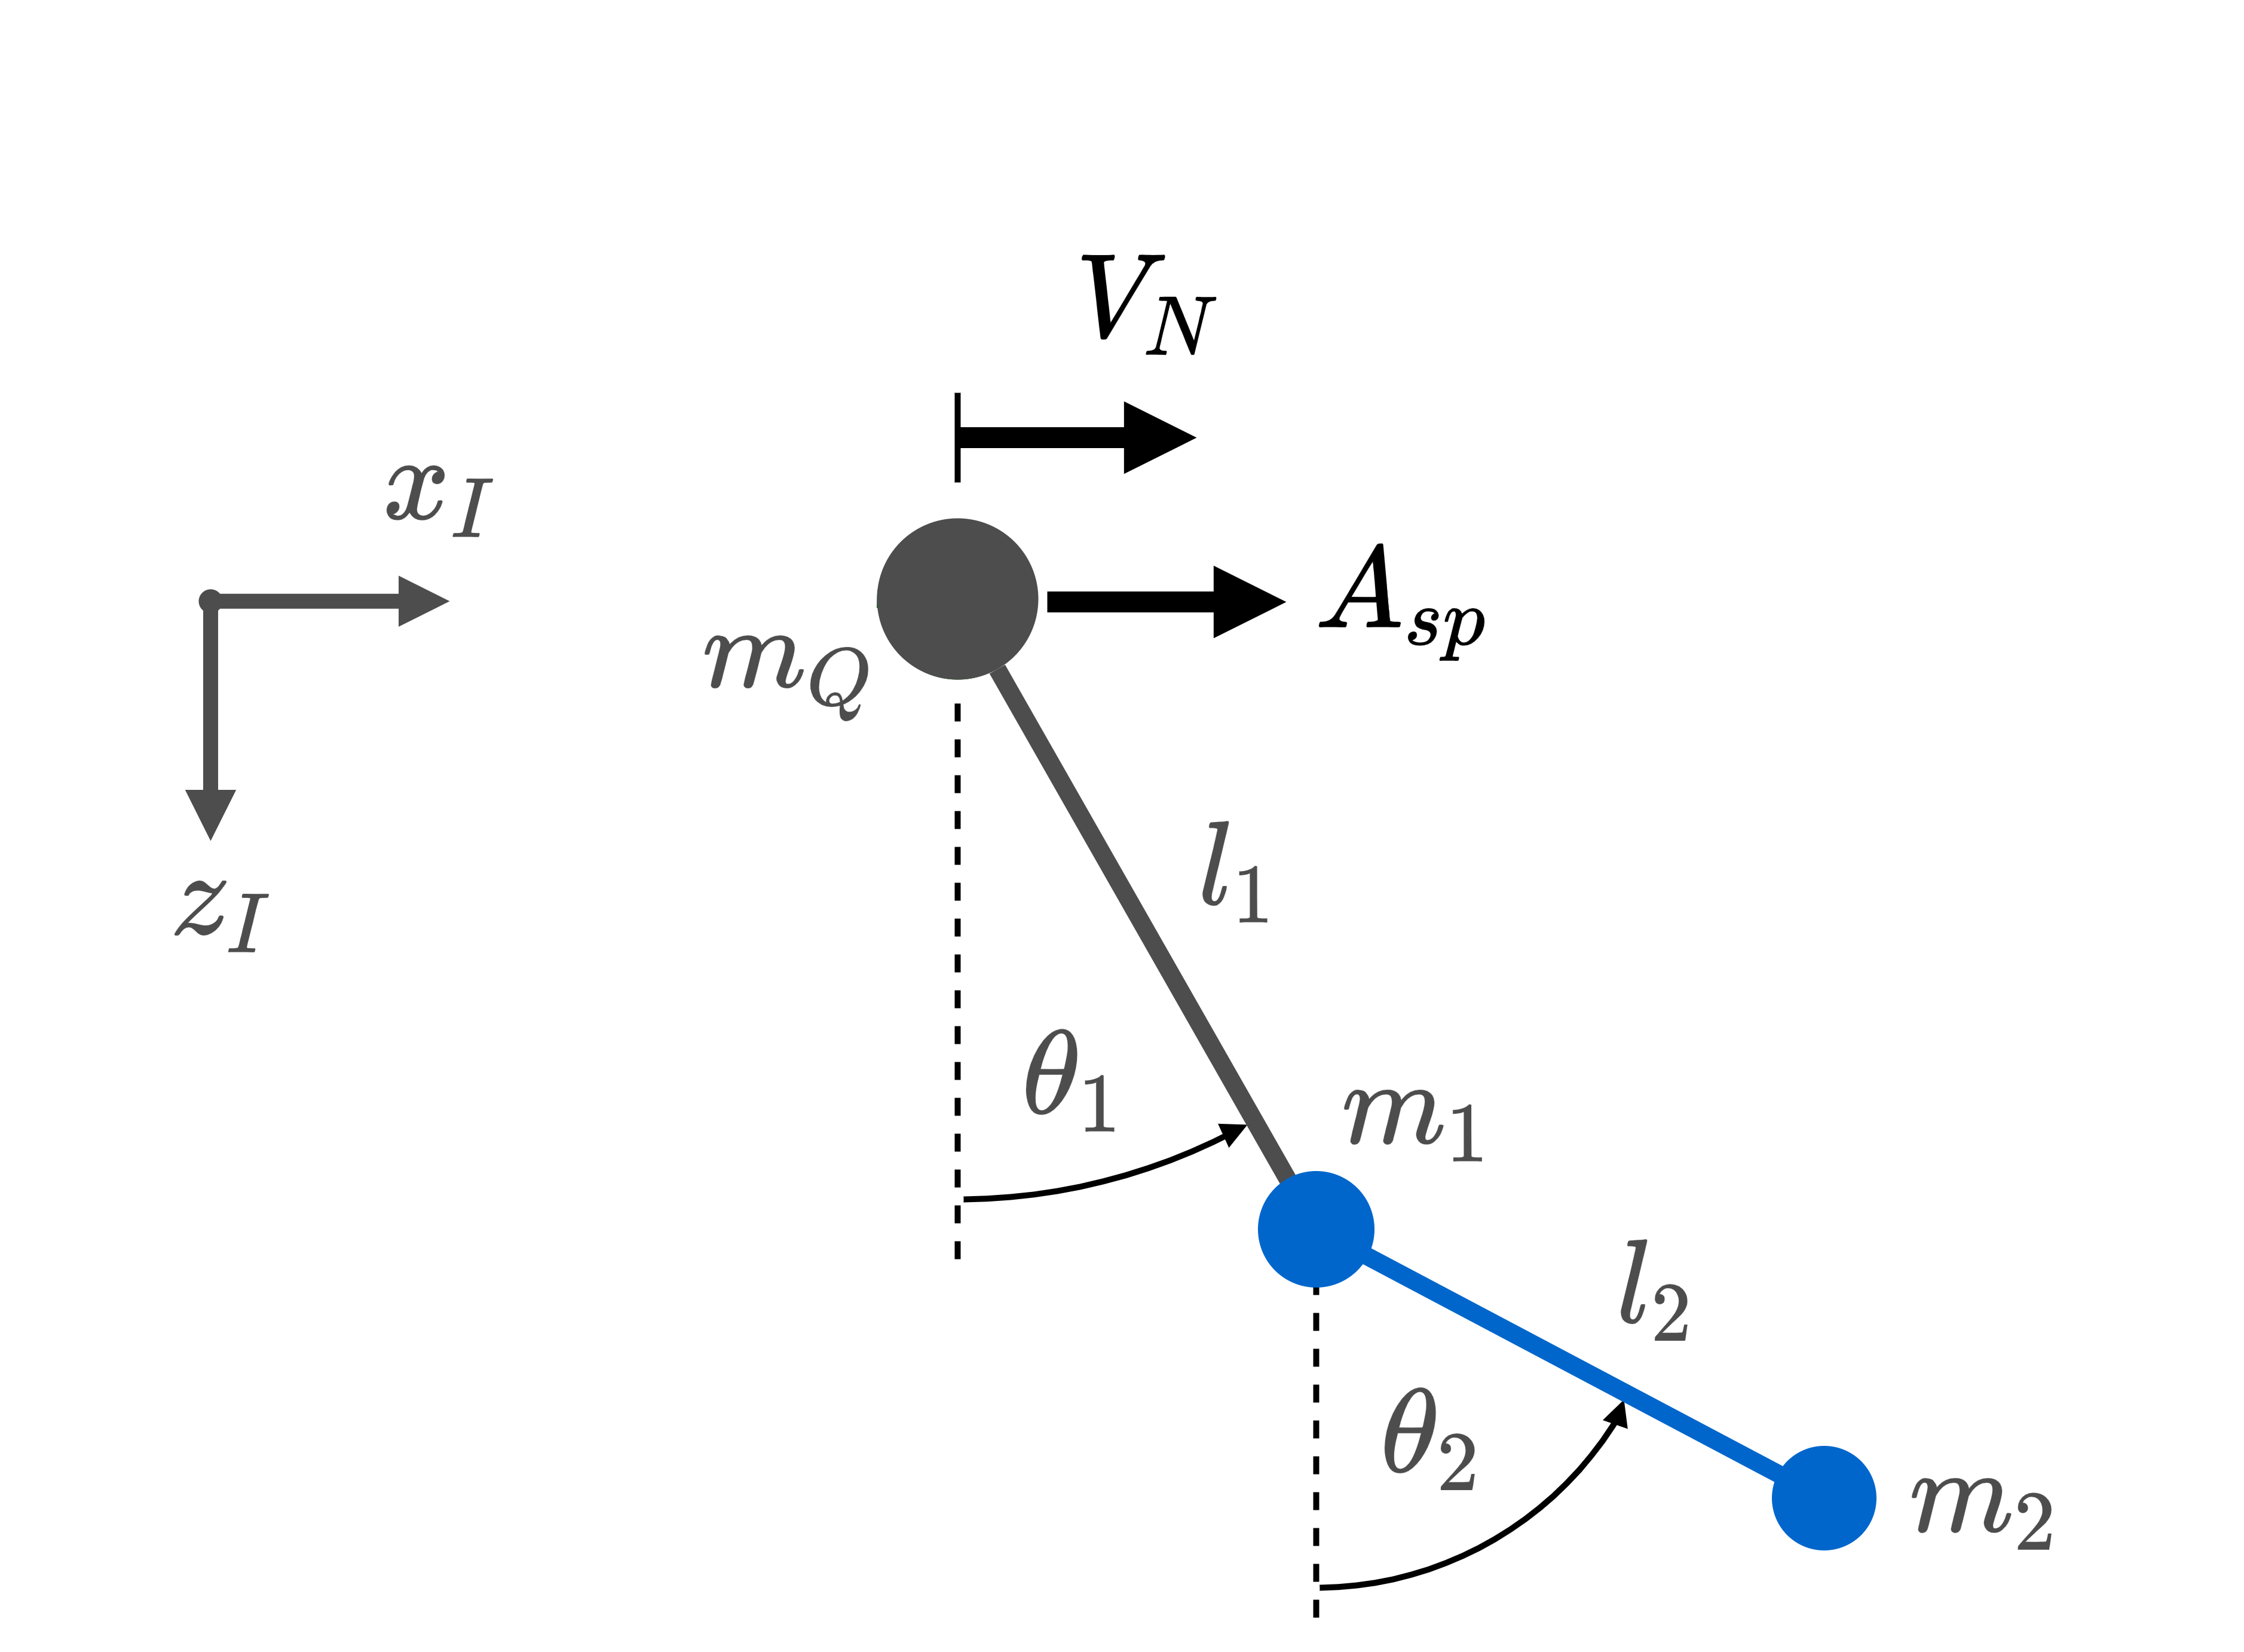
\includegraphics[width=0.5\linewidth]{double_pend.png}            
            \caption{Double pendulum model representing an elongated suspended payload}
            \label{fig:double_pend}
        \end{figure}
        
        % \paragraph
        % Figure~?? shows a practical double pendulum use case. 
        % \murray{insert picture a practical quad with long payload} ??
        % \murray{insert diagram of double pend}
        
        \paragraph
        Figure~\ref{fig:prediction_single_pend_white} shows the k-step-ahead prediction 
        of a white-box models for a single pendulum simulation.
        The exact $m_p$ is used for the model, but the cable length is estimated from a \gls{FFT} of the payload swing angle 
        as described in Section~\ref{sec:length_estimation}.
        It is clear that the prediction is accurate for the first few oscillations, 
        but the slight difference in frequency accumulates over time causing an increasingly large offset.
        However, the general shape of the dynamics is still captured by the model.
        Also note that the prediction oscillations are damped linearly 
        but the actual oscillations experience non-linear damping.
        This difference is an approximation error because the non-linear plant is modelled with a linear model. 

        \begin{figure}[htb]
    \centering
    \begin{tikzpicture}
        \begin{axis}[            
            xlabel = Time,
            ylabel = Payload angle,
            x unit = \si{\second},
            y unit = \si{\degree},
            xmin = 0,   xmax = 20,
            ymin = -12,  ymax = 6,
            grid = major,
            legend cell align = left,
            legend pos = north east,
            grid style = dashed,
            legend style = {font = \scriptsize},
            label style = {font = \scriptsize},
            tick label style = {font = \scriptsize},
            width = 0.95\columnwidth,
            height = 0.5\columnwidth,
            % initialize Dark2
            cycle list/Dark2,
            % combine it with 'mark list*':
            cycle multiindex* list = {
                Dark2\nextlist
            }
        ]
        
        \addplot+[mark = none, style = solid, ultra thick] 
        table[x = time, y expr = \thisrow{theta} * 57.2958, col sep = comma] 
        {system_id/csv/single_step_predictions_SITL_x_vel_noise_l1_m0-3.csv.csv};
        \addlegendentry{Actual}

        % \addplot+[mark = none, style = dashed, ultra thick] 
        % table[x = time, y = theta_dmd, col sep = comma] 
        % {system_id/csv/single_step_predictions_SITL_x_vel_noise_l1_m0-3.csv.csv};
        % \addlegendentry{DMDc}

        % \addplot+[mark = none, style = dashed, ultra thick] 
        % table[x = time, y = theta_havok, col sep = comma] 
        % {system_id/csv/single_step_predictions_SITL_x_vel_noise_l1_m0-3.csv.csv};
        % \addlegendentry{HAVOK}

        \addplot+[mark = none, style = dashed, ultra thick] 
        table[x = time, y expr = \thisrow{theta_white} * 57.2958, col sep = comma] 
        {system_id/csv/single_step_predictions_SITL_x_vel_noise_l1_m0-3.csv.csv};
        \addlegendentry{White-box}

        \end{axis}
    \end{tikzpicture} 
    
    \caption{White-box model predictions of a single pendulum for a North velocity step input
    ($l =$~\SI{1}{\metre}, $m_p =$~\SI{0.3}{\kilo\gram}).}
    \label{fig:prediction_single_pend_white}
\end{figure}

        
        \paragraph
        Figure~\ref{fig:prediction_double_pend_white} also shows the k-step-ahead prediction 
        of a white-box model, but this prediction is for a double pendulum simulation.
        The cable length was estimated from the same method 
        by calculating the \gls{FFT} of the cable swing angle and identifying the dominant frequency.
        Note how the prediction of the first oscillation is quite accurate and is similar to the initial swing of the single pendulum.
        However, by the second swing, the double pendulum dynamics differ significantly from the model prediction.
        The single pendulum oscillations seen in Figure~\ref{fig:prediction_single_pend_white} are regular
        compared to double pendulum oscillations in Figure~\ref{fig:prediction_double_pend_white} which are noticeably irregular.
        The a priori model expects regular, single frequency oscillations.
        This can be seen in Figure~\ref{fig:prediction_double_pend_white} where the predicted peaks are equidistant.
        However, the actual dynamics have a superposition of two frequencies due to the double pendulum payload.

        \begin{figure}[h]
    \centering
    \begin{tikzpicture}
        \begin{axis}[            
            xlabel = Time,
            ylabel = Payload angle,
            x unit = \si{\second},
            y unit = \si{\radian},
            xmin = 2,   xmax = 30,
            ymin = -0.2,  ymax = 0.2,
            grid = major,
            legend cell align = left,
            legend pos = north east,
            grid style = dashed,
            legend style = {font = \scriptsize},
            label style = {font = \scriptsize},
            tick label style = {font = \scriptsize},
            width = 0.95\columnwidth,
            height = 0.5\columnwidth,
            % initialize Dark2
            cycle list/Dark2,
            % combine it with 'mark list*':
            cycle multiindex* list = {
                Dark2\nextlist
            }
        ]
        
        \addplot+[mark = none, style = solid, ultra thick] 
        table[x = time, y = theta, col sep = comma] 
        {system_id/csv/single_step_predictions_SITL_single_vel_step_m1_0.2_l1_m2_0.1_l2_0.3.csv.csv};
        \addlegendentry{Actual}

        % \addplot+[mark = none, style = dashed, ultra thick] 
        % table[x = time, y = theta_dmd, col sep = comma] 
        % {system_id/csv/single_step_predictions_SITL_single_vel_step_m1_0.2_l1_m2_0.1_l2_0.3.csv.csv};
        % \addlegendentry{DMD}

        % \addplot+[mark = none, style = dashed, ultra thick] 
        % table[x = time, y = theta_havok, col sep = comma] 
        % {system_id/csv/single_step_predictions_SITL_single_vel_step_m1_0.2_l1_m2_0.1_l2_0.3.csv.csv};
        % \addlegendentry{HAVOK}

        \addplot+[mark = none, style = dashed, ultra thick] 
        table[x = time, y = theta_white, col sep = comma] 
        {system_id/csv/single_step_predictions_SITL_single_vel_step_m1_0.2_l1_m2_0.1_l2_0.3.csv.csv};
        \addlegendentry{White-box}

        \end{axis}
    \end{tikzpicture} 
    
    \caption{White-box model predictions of a double pendulum for a North velocity step input
        ($m =$~\SI{0.3}{\kilo\gram}, $l =$~\SI{1}{\meter})}
    \label{fig:prediction_double_pend_white}
\end{figure}

        
        \paragraph
        The \gls{FFT} amplitude spectrum of the single pendulum is shown in Figure~\ref{fig:FFT_double_pend}.
        This plot shows a single peak which corresponds to the natural frequency of the suspended payload.
        Figure~\ref{fig:FFT_single_pend} shows the \gls{FFT} amplitude spectrum of the double pendulum.
        Two peaks are revealed in this plot 
        which correspond to the two superimposed frequencies caused by the double pendulum.
        The frequency content of the two plants are clearly different 
        so the white-box model and parameter estimation techniques would need to be redesigned for these payloads specifically.
        This is the great disadvantage of the white-box system identification technique.
        For every model with different dynamics, a new technique needs to be designed and used.
        In contrast, the proposed data-driven method provides a general solution 
        for a large range of different payloads and dynamics.

        % The \gls{FFT} of the single pendulum leads to an estimated cable length of \SI{1.19}{\metre}        
        % The \gls{FFT} of the double pendulum leads to an estimated cable length of \SI{1.39}{\metre}
        
        
\begin{figure}
    \captionsetup[subfigure]{justification=centering}
    \centering
    \begin{subfigure}{0.45\columnwidth}
    \centering
    \begin{tikzpicture}
        \begin{axis}[            
            xlabel = Frequency,
            ylabel = Amplitude,
            x unit = \si{\radian/\second},
            % y unit = \si{\second},
            xmin = 0.3,     xmax = 1,
            ymin = 0,  ymax = 0.012,
            grid = major,
            legend cell align = left,
            legend pos = north east,
            grid style = dashed,
            legend style = {font = \scriptsize},
            label style = {font = \scriptsize},
            tick label style = {font = \scriptsize},
            width = 0.95\columnwidth,
            height = 0.95\columnwidth,
            % initialize Dark2
            cycle list/Dark2,
            % combine it with 'mark list*':
            cycle multiindex* list = {
                Dark2\nextlist
            }
        ]

        \addplot+[mark = none, style = solid, ultra thick] 
        table[x = f, y = P1, col sep = comma] 
        {system_id/csv/FFT_SITL_single_pos_step_m0.3_l1.csv.csv};

        \end{axis}
    \end{tikzpicture} 
    
    \caption{Single pendulum}
    \label{fig:FFT_single_pend}
\end{subfigure}
 % subfigure
    \begin{subfigure}{0.45\columnwidth}
    \centering
    \begin{tikzpicture}
        \begin{axis}[            
            xlabel = Frequency,
            ylabel = Amplitude,
            x unit = \si{\radian/\second},
            % y unit = \si{\second},
            xmin = 0.3,  xmax = 1,
            ymin = 0,    ymax = 0.012,
            grid = major,
            legend cell align = left,
            legend pos = north east,
            grid style = dashed,
            legend style = {font = \scriptsize},
            label style = {font = \scriptsize},
            tick label style = {font = \scriptsize},
            width = 0.95\columnwidth,
            height = 0.95\columnwidth,
            % initialize Dark2
            cycle list/Dark2,
            % combine it with 'mark list*':
            cycle multiindex* list = {
                Dark2\nextlist
            }
        ]

        \addplot+[mark = none, style = solid, ultra thick] 
        table[x = f, y = P1, col sep = comma] 
        {system_id/csv/FFT_SITL_single_pos_step_m1_0.2_l1_m2_0.1_l2_0.3.csv.csv};

        \end{axis}
    \end{tikzpicture} 
    
    \caption{Double pendulum}
    \label{fig:FFT_double_pend}
\end{subfigure}
 % subfigure
    \caption{ The single-sided amplitude spectrum of the swing angle FFT 
    ($m =$~\SI{0.3}{\kilo\gram}, $l =$~\SI{1}{\meter}).}
    \label{fig:FFT_subfigs}  
\end{figure}

        \paragraph
        Figure~\ref{fig:prediction_single_pend_black} shows the prediction of the two data-driven methods
        for a single pendulum simulation.
        Note that there is less of a frequency difference in this prediction than the white-box prediction in 
        Figure~\ref{fig:prediction_single_pend_white}.
        The shape of the predicted damping is also more similar to the actual dynamics than the white-box prediction.
        This may be because the data-driven methods effectively fit a higher order damping model to the dynamics,
        compared to the simple, linear damping applied in the white-box model.

        \paragraph
        The damping seen in these plots is a complicated effect which depends on 
        the payload connection, 
        the aerodynamic drag, 
        and
        the controller gains.
        An advantage of data-driven system identification techniques 
        is that the effect of damping is inherently included in the estimated model 
        without specifically estimating a damping coefficient.
        In contrast, the white-box estimation technique requires the effect to be modelled a priori 
        and a designed algorithm to estimate every parameter that effects the dynamics.

        \begin{figure}[htb]
    \centering
    \begin{tikzpicture}
        \begin{axis}[            
            xlabel = Time,
            ylabel = Payload angle,
            x unit = \si{\second},
            y unit = \si{\radian},
            xmin = 0,   xmax = 20,
            ymin = -0.2,  ymax = 0.1,
            grid = major,
            legend cell align = left,
            legend pos = north east,
            grid style = dashed,
            legend style = {font = \scriptsize},
            label style = {font = \scriptsize},
            tick label style = {font = \scriptsize},
            width = 0.95\columnwidth,
            height = 0.5\columnwidth,
            % initialize Dark2
            cycle list/Dark2,
            % combine it with 'mark list*':
            cycle multiindex* list = {
                Dark2\nextlist
            }
        ]
        
        \addplot+[mark = none, style = solid, ultra thick] 
        table[x = time, y = theta, col sep = comma] 
        {system_id/csv/single_step_predictions_SITL_x_vel_noise_l1_m0-3.csv.csv};
        \addlegendentry{Actual}

        \addplot+[mark = none, style = solid, ultra thick] 
        table[x = time, y = theta_dmd, col sep = comma] 
        {system_id/csv/single_step_predictions_SITL_x_vel_noise_l1_m0-3.csv.csv};
        \addlegendentry{DMD}

        \addplot+[mark = none, style = dashed, ultra thick] 
        table[x = time, y = theta_havok, col sep = comma] 
        {system_id/csv/single_step_predictions_SITL_x_vel_noise_l1_m0-3.csv.csv};
        \addlegendentry{HAVOK}

        % \addplot+[mark = none, style = dashed, ultra thick] 
        % table[x = time, y = theta_white, col sep = comma] 
        % {system_id/csv/single_step_predictions_SITL_x_vel_noise_l1_m0-3.csv.csv};
        % \addlegendentry{White-box}

        \end{axis}
    \end{tikzpicture} 
    
    \caption{Data-driven model predictions of a single pendulum for a North velocity step input
        ($m =$~\SI{0.3}{\kilo\gram}, $l =$~\SI{1}{\meter}).}
    \label{fig:prediction_single_pend_black}
\end{figure}
        
        
        \paragraph
        Figure~\ref{fig:prediction_double_pend_black} shows the prediction of the same data-driven methods 
        but for a double pendulum simulation.
        The same cable length and effective payload mass is used here as in the single pendulum simulation.
        Notice how accurate the prediction is for the first \SI{20}{\second} of the plot.
        In contrast to the white-box model, the black-box model oscillations follow the irregular, 
        multi-frequency response of the actual dynamics.
        The state-space model can approximate the multi-frequency dynamics of the plant 
        because of the delay-coordinates in the model.
        As expected, the prediction accuracy is also much better than the white-box models 
        for both the single and double pendulum simulations. 

        \begin{figure}[htb]
    \centering
    \begin{tikzpicture}
        \begin{axis}[            
            xlabel = Time,
            ylabel = Payload angle,
            x unit = \si{\second},
            y unit = \si{\degree},
            xmin = 2,   xmax = 30,
            ymin = -12.0,  ymax = 6,
            grid = major,
            legend cell align = left,
            legend pos = north east,
            grid style = dashed,
            legend style = {font = \scriptsize},
            label style = {font = \scriptsize},
            tick label style = {font = \scriptsize},
            width = 0.95\columnwidth,
            height = 0.5\columnwidth,
            % initialize Dark2
            cycle list/Dark2,
            % combine it with 'mark list*':
            cycle multiindex* list = {
                Dark2\nextlist
            }
        ]
        % y expr = \thisrow{} * 57.2958
        \addplot+[mark = none, style = solid, ultra thick] 
        table[x = time, y expr = \thisrow{theta} * 57.2958, col sep = comma] 
        {system_id/csv/single_step_predictions_SITL_single_vel_step_m1_0.2_l1_m2_0.1_l2_0.3.csv.csv};
        \addlegendentry{Actual}

        \addplot+[mark = none, style = solid, ultra thick] 
        table[x = time, y expr = \thisrow{theta_dmd} * 57.2958, col sep = comma] 
        {system_id/csv/single_step_predictions_SITL_single_vel_step_m1_0.2_l1_m2_0.1_l2_0.3.csv.csv};
        \addlegendentry{DMDc}

        \addplot+[mark = none, style = dashed, ultra thick] 
        table[x = time, y expr = \thisrow{theta_havok} * 57.2958, col sep = comma] 
        {system_id/csv/single_step_predictions_SITL_single_vel_step_m1_0.2_l1_m2_0.1_l2_0.3.csv.csv};
        \addlegendentry{HAVOK}

        % \addplot+[mark = none, style = dashed, ultra thick] 
        % table[x = time, y = theta_white, col sep = comma] 
        % {system_id/csv/single_step_predictions_SITL_single_pos_step_m1_0.2_l1_m2_0.1_l2_0.3.csv.csv};
        % \addlegendentry{White-box}

        \end{axis}
    \end{tikzpicture} 
    
    \caption{Data-driven model predictions of a double pendulum for a North velocity step input
        ($m_1 =$~\SI{0.2}{\kilo\gram}, $l_1 =$~\SI{1}{\meter}, $m_2 =$~\SI{0.1}{\kilo\gram}, $l_2 =$~\SI{0.3}{\meter})}
    \label{fig:prediction_double_pend_black}
\end{figure}

        
        \paragraph
        The double pendulum plant involves a hidden state variable, 
        because the unmeasured angle of the second pendulum 
        is required to fully describe the state of the system.
        However, the \gls{DMDc} and \gls{HAVOKc} models are still able to approximate the dynamics quite accurately 
        without measuring this state variable.
        This is due to the extent of the delay embedding of the models \cite{Kamb2020}.
        Figure~\ref{fig:MAE_vs_q_double_pend} shows the prediction error 
        as a function of the number of delays in the model for a double pendulum.
        Note how much more delays is required before the prediction error reaches steady-state 
        than for a single pendulum showed in Figure~\ref{fig:NMAE_vs_q}.
        This is because the dynamics are more complex 
        and model needs a lot more parameters to account for the hidden state variable.
        % Also note that \gls{HAVOKc} seems to mostly produces slightly lower errors for low values of $q$,
        % but \gls{DMDc} and \gls{HAVOKc} produce very similar
                
        \begin{figure}[htb]
    \centering
    \begin{tikzpicture}
        \begin{axis}[            
            xlabel = {Number of delay-coordinates, $q$},
            ylabel = $\overline{NMAE}$ \phantom{~},
            % x unit = \si{\second},
            y unit = \%
            xmin = 6,     xmax = 50,
            ymin = 3,  ymax = 6.5,
            grid = major,
            legend cell align = left,
            legend pos = north east,
            grid style = dashed,
            legend style = {font = \scriptsize},
            label style = {font = \scriptsize},
            tick label style = {font = \scriptsize},
            width = 0.95\columnwidth,
            height = 0.5\columnwidth,
            % initialize Dark2
            cycle list/Dark2,
            % combine it with 'mark list*':
            cycle multiindex* list = {
                Dark2\nextlist
            }
        ]
        
        \addplot+[mark = none, style = solid, ultra thick] 
        table[x = q, y expr = {\thisrow{NMAE_mean}*100}, col sep = comma] 
        {system_id/csv/NMAE_vs_q_SITL_x_vel_noise_m1_0.2_l1_m2_0.1_l2_0.3_Train_70.csv_dmd_angle.csv};
        \addlegendentry{DMD}
        
        \addplot+[mark = none, style = solid, ultra thick] 
        table[x = q, y expr = {\thisrow{NMAE_mean}*100}, col sep = comma] 
        {system_id/csv/NMAE_vs_q_SITL_x_vel_noise_m1_0.2_l1_m2_0.1_l2_0.3_Train_70.csv_havok_angle.csv};
        \addlegendentry{HAVOK}

        \end{axis}
    \end{tikzpicture} 
    
    \caption{\gls{DMD} and \gls{HAVOK} predictions error of double pendulum for different numbers of delay-coordinates
    ($m_1 =$~\SI{0.2}{\kilo\gram}, $l_1 =$~\SI{1}{\meter}, $m_2 =$~\SI{0.1}{\kilo\gram}, $l_2 =$~\SI{0.3}{\meter} $T_{train} =$~\SI{70}{\second}.)}
    \label{fig:MAE_vs_q_double_pend}
\end{figure}


        \paragraph
        Overall, the data-driven system identification approaches were shown to work well 
        for both the single and double pendulum payloads.
        In contrast, the white-box method describes the general shape of the single pendulum dynamics well, 
        but do not perform well for a double pendulum simulation 
        because it was specifically designed for the single pendulum payload.
        The data-driven approaches therefore provide an accurate system identification method 
        for a much larger range of payload types without needing a redesign for specific payload dynamics.
        
        % ?? plot q of single pend on the same axis

        % \begin{figure}[htb]
    \centering
    \begin{tikzpicture}
        \begin{axis}[            
            xlabel = Length of training data,
            ylabel = $\overline{NMAE}$ \phantom{~},
            x unit = \si{\second},
            y unit = \%,
            xmin = 0,     xmax = 90,
            ymin = 6,  ymax = 15,
            grid = major,
            legend cell align = left,
            legend pos = north east,
            grid style = dashed,
            legend style = {font = \scriptsize},
            label style = {font = \scriptsize},
            tick label style = {font = \scriptsize},
            width = 0.95\columnwidth,
            height = 0.5\columnwidth,
            % initialize Dark2
            cycle list/Dark2,
            % combine it with 'mark list*':
            cycle multiindex* list = {
                Dark2\nextlist
            }
        ]
        
        \addplot+[mark = none, style = solid, ultra thick] 
        table[x = T_train, y expr = {\thisrow{NMAE_mean}*100}, col sep = comma] 
        {system_id/csv/NMAE_vs_Ntrain_SITL_x_vel_noise_l1_m0-3.csv_havok_angle.csv};
        \addlegendentry{single pendulum - $m_p =$~\SI{0.3}{\kilo\gram}, $l =$~\SI{1}{\metre},}
        
        \addplot+[mark = none, style = solid, ultra thick] 
        table[x = T_train, y expr = {\thisrow{NMAE_mean}*100}, col sep = comma] 
        {system_id/csv/NMAE_vs_Ntrain_SITL_x_vel_noise_m1_0.2_l1_m2_0.1_l2_0.3.csv_havok_angle.csv};
        \addlegendentry{double pendulum - $m_1 =$~\SI{0.2}{\kilo\gram}, $m_1 =$~\SI{0.1}{\kilo\gram}, $l_1 =$~\SI{1}{\metre}, $l_2 =$~\SI{0.3}{\metre}}
        
        \end{axis}
    \end{tikzpicture} 
    
    \caption{\gls{HAVOKc} prediction error using different cable lengths with a range of different lengths of noisy training data
    ($l =$~\SI{1}{\metre}, $T_{train} =$~.).}
    \label{fig:single_vs_double_pend}
\end{figure}


        % \paragraph
        % The double pendulum is one example of a payload case that would require a redesign of the control architecture.
        % Other dynamic payloads that are difficult to model with a white-box method are containers holding a fluid.
        % Examples: 

        % \paragraph
        % Another payload case that will cause inaccuracies in estimated white-box model 
        % is if a payload is attached rigidly to the multirotor while also carrying a suspended payload.
        % The payload mass estimation is based on the assumption that the multirotor mass is known.
        % However if a mass is rigidly attached to the vehicle, the effective multirotor mass is changed and the \gls{RLS} payload mass estimation is no longer accurate.
        
        % \paragraph
        % To determine whether the white-box or data-driven methods perform better with these payloads, 
        % the performance of these methods need to be compared to each other.
        % However, comparing these methods is a non-trivial task
        % because they result in different types of models which are used in different types of controllers.
        % The white-box system identification technique generates a continuous-time, state space model 
        % which is used in an \gls{LQR} controller. 
        % This is in the form:
        % \begin{equation}
        %     \dot{x} = A x + B u
        % \end{equation}
        % For this model, the accuracy of the time-derivative estimate  
        % at the current time-step is important for control.
        % Hence, a k-step-ahead prediction error is not a good measure of performance for this model.
        % In contrast, the data-driven techniques result in a discrete state space model,
        % \begin{equation}
        %     x_{k+1} = A x_k + B u_k ,
        % \end{equation} 
        % which is used in a \gls{MPC}.
        % The k-step-ahead prediction accuracy of this model is important for the performance of the \gls{MPC}.
        % Therefore comparing the performance of the controllers which use these models 
        % is a better approach than comparing the model accuracy.
        % This will be investigated in Chapter~\ref{chap:control}.

